\section{A little fun in the valleys south of the bivi}

\begin{marginfigure}
\begin{tikzpicture}
\node [name-dest] (box){%
    \begin{minipage}{0.80\textwidth}
     \begin{itemize}
    \item Will Scott
    \item Tanguy Racine
    \end{itemize}
    \end{minipage}

};
\node[fancytitle, right=10pt] at (box.north west) {TR01 - a little ice cave};
\end{tikzpicture}
\end{marginfigure}

The Limestone pavement: a region that hasn’t received much attention in the past decade. This ‘flat bottomed’ feature is truly remarkable: covering an ellipse of semi-axes 100m and 200m, oriented NW-SE, it lies between the Bivi and the peak of Migovec. The dip of the beds in this area is towards the south -west, therefore exposing bedding as steps ranging from 1.5 to 2m. On the surface, two perpendicular arrays of linear joints are exposed and enlarged by precipitation and snowmelt, forming elongate pits choked with snow and ice abound in the area. This makes cave prospection difficult. This area is the true southern part of the plateau, hosting the 110m deep pot of PF10.  At depth, this is where the ramifications and active streamways of the Atlantis branch were found. Could this region provide entry from above into the southern extensions?

\begin{marginfigure}
\centering
\frame{\includegraphics[width=\linewidth]{"images/2016/tanguy-pavement-2016/migface_narrow".jpg}}
\label{migface}
\caption{On an airy spur of rock, the view of the Migovec cliff face reveals a hunter's path with voids above and below, snaking past several massive buttresses --- Tanguy Racine}
\end{marginfigure}

I had managed to reconnoitre the area in 2014, following Jarvist’s advice that little else than PF10 had been discovered. On my own, I packed a small bag with GPS, gloves, light and oversuit to check out as many likely holes as possible. This was a foggy day and I logged 8 caves or beginnings thereof that I had visited. Some died conclusively as the wall rock closed down on the passage, some I hadn’t got rope to descent, others choked with ice and scree. One I got slightly stuck in, for want of digging enough scree out of small squeeze. As I advanced the rotation of the cobbles denied the possibility to back out. 

The only way was forward, into a small aven chamber which died immediately. Shimmying forward got me unstuck but the ordeal highlighted how unwise it was to go too far on one’s own. When I got out, the fog was thick, the breeze cool, and unbidden thoughts about one’s vulnerability up in the mountains sprung to my mind. I carried on with my search more cautiously. In the end, there was one cave I’d spotted (several entrances, including an aven) that had grabbed my attention. Unfortunately I lacked the rope to descend it on the day, and for another two years it waited.

As it happened, Will, Arun, Kenneth and I planned to go back down to Tolmin mid-expedition. The day before going down there seemed to be a lot of agitation in the bivi. Recent finds of large chambers, horizontal passages and shaft series had gripped the imagination of the group. Little few cavers remained on the surface on the day, but among those Will Scott helped Janet, Dave and I cleaning and clearing the Bivi (not in that order). With the sunshine, an afternoon ramble across the plateau with a light caving bag seemed reasonable. With the morning chores completed and plans for the day finalised Janet Will and I set off, trodding the ‘old Mig path’ Janet had been trimming and clearing up after several years. 

From the Bivi it led along the top of the M16 escarpment, gently curving to the SE. Gardener’s World Valley and Area S unfolded in front of us, then in the distance we spotted the Razor hut, and further still a line of limestone crested mountains heading south, till they disappeared in the haze. This panorama was a feast of soft greens, greys and blues. At the end of the clear path, we turned due south towards the peak of Migovec, going across a grassy, hilly terrain, circumnavigating the shakeholes. On our right, we passed the Amphitheatre, a large 50m wide depression with excellent acoustics. On the verge of the Limestone Pavement, the ground dropped steeply forcing up to pick a snaking path towards the head of the valley, past some of the rare trees of the Plateau that do not appear to suffer from dwarfism. 

\begin{figure*}[t!]
\checkoddpage \ifoddpage \forcerectofloat \else \forceversofloat \fi
    \centering
    \begin{subfigure}[t]{0.59\textwidth}
        \centering
        \frame{\includegraphics[width=\linewidth]{"images/2016/tanguy-pavement-2016/WillScott-bolting".jpg}} 
        \caption{} \label{Will Scott bolting}
    \end{subfigure}
    \hfill
    \begin{subfigure}[t]{0.393\textwidth}
        \centering
        \frame{\includegraphics[width=\linewidth]{"images/2016/tanguy-pavement-2016/Janet_Pavement".jpg}} 
        \caption{} \label{Ice}
    \end{subfigure}

    \vspace{0.3cm}
    \begin{subfigure}[t]{\textwidth}
    \centering
        \frame{\includegraphics[width=\linewidth]{"images/2016/tanguy-pavement-2016/View_of_Razor".jpg}} 
        \caption{} \label{Panorama}
    \end{subfigure}
    \caption{
    \emph{a} The entrance pitch to TR01, hand bolted by Will Scott
    \emph{b} Janet Cotter enjoying a snack on the Limestone Pavement
    \emph{c} The panorama from the Eastern Promontory, by the 'old mig path' showing the Razor alp and the refuge --- Tanguy Racine }
\end{figure*}


The Pavement was as I remembered, bare limestone beds, deep shady cold pits exhaling their cold breath. We kept to the northern, deeper end of the valley, choosing a careful path amidst the boulders. With the GPS we found the cave of interest quickly, had a look and pressed on ‘downstream’ - the pavement is a hanging valley, completely dry. 

This led to M24, a depression of the same scale as the Amphitheatre, open to the north, boasting a 20x20m snowplug. At the far deep end of the shake hole, a small rift could be entered, a rift that dies within five metres, choked with boulders. On the eastern cliff face  (I am using this word here because of the asymmetrical nature of the depression), a large entrance to a cavity could be seen. It is certainly possible to climb into it and drop a rope for safety, but it is unclear whether this would only take one up into a small shaft that once led into a cavern. 

Past M24, we found the ‘old mig path’ again, in much better state than a completely abandoned trail would be. Cuts on the trees were old, maybe two or three years, but no more. I understand that it was once the highway from Kal to the Plateau, creeping up the eastern rather than the western slopes of the mountain. It must cross the Mig southern cliff face. Some 200 to 300 metres of decaying limestone, and underneath a high angle scree slope, funnelled into a couple of dry valleys. All the way to Ravne. 

Indeed the path led to the start of a vertigo-inducing traverse of face of Migovec, but before that it took us to a gorgeous panoramic from the high eastern promontory. All that we had seen before and more unfolded before our eyes, from Skrbina to Zabiski Kuk, thence down to Tolmin and up to Grusnica. And everything beyond, Most-na-Soci, the plain of Trieste. Most of all, the entire bowl of the Razor alp, the southern apron of Migovec where Coincidence cave lies, all of it crystal clear. A crow’s nest. We turned around after a few minutes of silent contemplation and climbed back up to TR01, the cave in waiting. 

It took only a few minutes for Will to learn how to hand bolt. I demonstrated first placing the back up bolt while he looked on. Janet sat on the pavement and shared the little treat she had brought along: crackers, jam, mountain cheese. Will put his kit on and got to work with a gentle tap tap tap tap  of the driver into the hard limestone. He acquitted himself very well and before long the only other bolt placement needed to complete the trivial descent of a 5 metre drop was done. Without effort he rigged the pitch and descended. I commanded him to remain silent, but a few ‘ohs’ and ‘ahs’ came back up. I followed quickly dropping into a small chamber.
‘It might not die immediately’ Will said, thereby attracting the anger of the cave deity. Though not all doors were closed, none went very far. 

\begin{marginfigure}
\centering
\frame{\includegraphics[width=\linewidth]{"images/2016/tanguy-pavement-2016/Bivi-chocolate".jpg}}
\label{chocolate}
\caption{The chocolate and sweets situation in the bivi is one of two extremes: pre-carry dearth or post-carry instant carnage --- Cecilia Kan}
\end{marginfigure}


\begin{figure*}[t!]
\checkoddpage \ifoddpage \forcerectofloat \else \forceversofloat \fi
    \centering
    \begin{subfigure}[t]{0.393\textwidth} %16:9
        \centering
        \frame{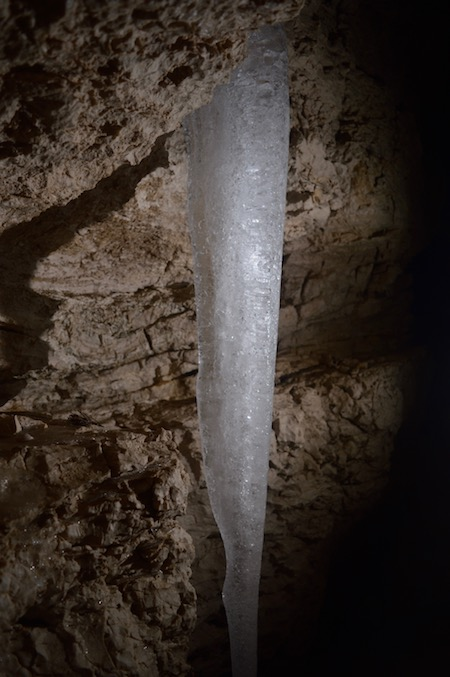
\includegraphics[width=\linewidth]{images/2016/tanguy-pavement-2016/Ice-2016.jpg}} 
        \caption{} \label{Ice stalactite}
    \end{subfigure}
    \hfill
    \begin{subfigure}[t]{0.59\textwidth} %square
        \centering
        \frame{\includegraphics[width=\linewidth]{"images/2016/tanguy-pavement-2016/Will_TR01".jpg}} 
        \caption{} \label{Will scott}
    \end{subfigure}

    \vspace{0.3cm}
    \begin{subfigure}[t]{\textwidth} %16:9
    \centering
        \frame{\includegraphics[width=\linewidth]{"images/2016/tanguy-pavement-2016/Ice_curtain".jpg}} 
        \caption{} \label{Ice curtain}
    \end{subfigure}
    \caption{
    \emph{a} The jewel of TR01 - A modest 1m ice stalactite
    \emph{b} Will Scott in the first snow plugged chamber
    \emph{c} An ice curtain found in one of the extensions --- Tanguy Racine }
\end{figure*}




The cave was by all accounts a small one. It sported a modest chamber, linked to an aven (5m) to the west, choked with ice and rubble. Right by the landing there was a draughting snowhole. At the far end of the chamber, a small tube, littered in wet, sharp pebbles led off for  a few metres in another chamber, of even smaller dimensions. The walls were covered in glittering ice, with a few curtains and stalactites (of ice) shining to our lights. I took a few photos, and proceeded to descend the snow hole. Will looked at me with a solemn face. Here goes another nutter he might have thought. We were in T-shirts, and the temperature within the cave, in the draught was not balmy. But wait, wasn’t it obvious? A snow hole, the draught, what massive chambers could lie beyond? I did not hesitate and descended.

Unfortunately the rope was at an angle to the tube of glistening wet snow, and started rubbing, then sawing, then hacking big chunks of snow down on me. Quickly I abseiled till my feet touched the floor. I put my weight on them and the floor went from under me, a pile of rubble flying out. I caught the rope, and pivoted to see what gigantic chamber I’d landed in. 

It was cosy, a 2metre wide rift, degenerating to next to nothing at all downwind, but it was worth it, for a glittering, metre long, thick carrot like stalactite hung from the righthand wall. It even had growth rings, refracting the light in all directions. I urged Will to come down. He absolutely had to see it. And he did, though he cursed me a little for the ice shower. I was not going to let him off for this, so I asked him to carry my flashgun in the most cramped positions imaginable, in the snow tubes that led off. The resulting play on light and shadow in the mini-wonderland was worth the effort. 



Back in the sunshine, we derigged the cave, ate the remaining crackers with Janet, and set off in search for PF10. Once the boulder-filled shakehole was located we carried on uphill towards the bivi and found the grassy N-S avenue which leads to camping site. Within minutes we were back in the fading sunlight at the top of the Plateau and headed to the Bivi where the dinner preparation awaited. Will and I also baked some cocoa and ground almond flapjacks, which earned the nickname ‘Tanguy Treats’. We were low on underground food, and this glorious enterprise averted a chocolate bar crisis. Donuts were deep fried and given to the earliest returning cavers. Jack and Kenneth, then Rhys and Arun and finally William and Miriam. Again there were tales of more horizontal passage and a typical late Bivi night. 



\begin{pagefigure}
\centering
\frame{\includegraphics[width=\linewidth]{"images/2016/tanguy-pavement-2016/icecave"}}
\caption{A hand drawn survey of TR01 with plan and elevation --- Tanguy Racine}
\label{scan}
\end{pagefigure}
\name{Tanguy Racine}

